\documentclass[letterpaper,11pt,twocolumn]{article}
\usepackage{usenix,graphicx,times}

%\usepackage{graphics, graphicx, fancyhdr, epsfig, amstext}
%\usepackage{amsmath, amssymb, xspace, setspace, times, color}

\begin{document}

\title{CSCI 339 Final Project: Peer-to-Peer Ride-Sharing} 
\date{}

\author{
  {\rm Erik Kessler, Kevin Persons}\\
       Williams College\\
}

\maketitle

\thispagestyle{empty}
%\pagestyle{empty}
                                   
\begin{abstract}
This paper describes the motivation, design, and evaluation of our distributed ridesharing platform. One goal of this project is to provide an easy to setup and customize testing environment allowing for the agile, iterative, and data driven development of a ridesharing protocol in a distributed peer-to-peer environment. We designed the simulator to allow experimenters to easily tune the simulation to model different real world scenarios to see how they should expect their protocol to behave. The second part of the project involved using our simulator to develop and test a scalable and performant peer-to-peer ridesharing  protocol that could serve as the basis for a real world ridesharing service.
\end{abstract}

\section{Introduction}
Recent years have shown the growth and expanding popularity of transportation networking applications such as Uber and Lyft. The public is becoming increasingly open to the idea of receiving rides from application-verified strangers and paying for these rides online. A related type of service that is also benefiting from this rapid shift is real-time ridesharing. The general idea behind real-time ridesharing is that a person willing to share a seat in their car can offer the seat to someone who is looking for a ride to the same place, either for free or for payment. The taxi industry and other organizations have begun to push back against all of these transportation services, and recently, policymakers have passed laws banning or limiting these services in certain areas.

Regardless of the politics, it is clear that there is a market for these kinds of services, and it seems like real-time ridesharing in particular could be especially useful in smaller communities like on a college campus. Thus, we were motivated to explore how one would develop a decentralized and community-owned real-time ridesharing service. The peer-to-peer file-sharing community, consisting of services like BitTorrent that have been highly resilient against takedown, provides good ideas on where to start. It is clear that a fully decentralized, peer-to-peer system is the best way to achieve these goals of takedown resistance and community ownership. An additional motivation and benefit of making ridesharing peer-to-peer is that there will not be a service providing company charging fees for use of their platform. In the scenario of a college campus this would likely be very desirable as students would be able to more readily participate as both drivers and passengers and the service would allow for informal payments like offers to share food.

Ridesharing, at its core, just involves matching users based on their locations and their status of seeking or offering a ride. These operations are straightforward to implement in a centralized system where a cluster of servers can receive location updates from all users, calculate the distance between potential matches, and then notify the best-matched pair with the location of the other user. In a peer-to-peer setting, however, this problem becomes more complex. With no central servers to manage the locations of all users, each peer in the network must coordinate its own exchanging of geolocation data with other peers and determine based only on its own view of the system whether it should match with another user. Due to the high cost of sending location update messages over the network, it is not feasible for every peer to be in frequent contact with every other peer, and so any given peer has only a limited perspective of the whole system when making matching decisions.

One important consideration for this project is that we are working in a mobile environment. This has a number of implications. For one, mobile devices have limited resources, so we want to limit the amount of computation and message sending we are doing. We don't want to waste the user's battery or other limited resources. Furthermore, mobile connections have less bandwidth, higher latency, and less reliability as users can lose service at anytime.   

Therefore, the goals of our system were to create a scalable system in that even as the 
number of users in the network grows, the amount of time and number of network messages it takes to perform an operation remains reasonable and usable. Also, using a term from Brewer's paper, we are aiming for high harvest. We want to make sure that our operations are working on a reasonably full set of the data so we aren't missing potential rides. 

The approach we take is influenced by the Chord paper. The Chord paper discussed how they used a simulator to test and evaluate their protocol. Since gathering a vast number of mobile devices and conducting real-world tests with them is outside the scope of this project, we needed an easier way to test our protocol. As a result, we decided to build a simulator which would allow us to control certain conditions, set up specific scenarios, and easily collect data for evaluation. 

\section{Architectural Overview}
Our project consists of two main parts: the simulator and the ridesharing protocol. We built the simulator in order to test and evaluate our implementation of the protocol, so we will first give an overview of the simulation environment. We will then discuss the design of our protocol implementation, the various tradeoffs involved, and how the design helps move us towards our goals of scalability and high harvest.

\subsection{Simulator}
Our main goal with the simulator was to provide a fast and low cost way to test how we should expect our service to perform in a real-world setting. Our simulator consists of two major components: a world and a list of peers.

For simplicity, we decided to model the world as a circular, one-dimensional line. We thought this would be a reasonable simplification to make because it would make every nearly every aspect of the simulator easier to reason about. Furthermore, the patterns that show up on a one-dimensional world should be similar to those of a two-dimensional world, and we could, eventually, expand the world to be two-dimensional if needed.

The peers are the users of the service that move around in the world and interact with each other. We modeled four types of peers: passengers who mainly sit still looking for rides, random movers who just move around, travelers who move long distances in one direction, and commuters who move back and forth between two locations. We designed the system so that if we wanted a new peer type in order to better model reality or some specific situation, it is very straightforward as we would simply override the peer base class and define a \texttt{stepAction} function that describes how the peer should move.

Each peer holds it current position, a list of known peers, and a log of recent action. The list of known peers is what allows this to be a peer-to-peer network. So instead of sending requests to a central server, all operations for the ridesharing service that the peer wants to perform will have to go through peers of this peer list. Thus, effectively maintaining, updating, and using this known peer list will be critical to the performance of the service. 

The simulator creates a list of different peer types and places them in the world. We created two different methods for initializing this peer list. The first way adds all peers to the world at once and initializes the known peer list of each node to be a random list of other peers. The other way provides a more real world initialization. We add peers one by one, and each peer starts out knowing about only one other peer. This is more realistic, because in reality someone would join the network by learning about some other person already in the network.

\begin{figure*}[ht]
  \centering
   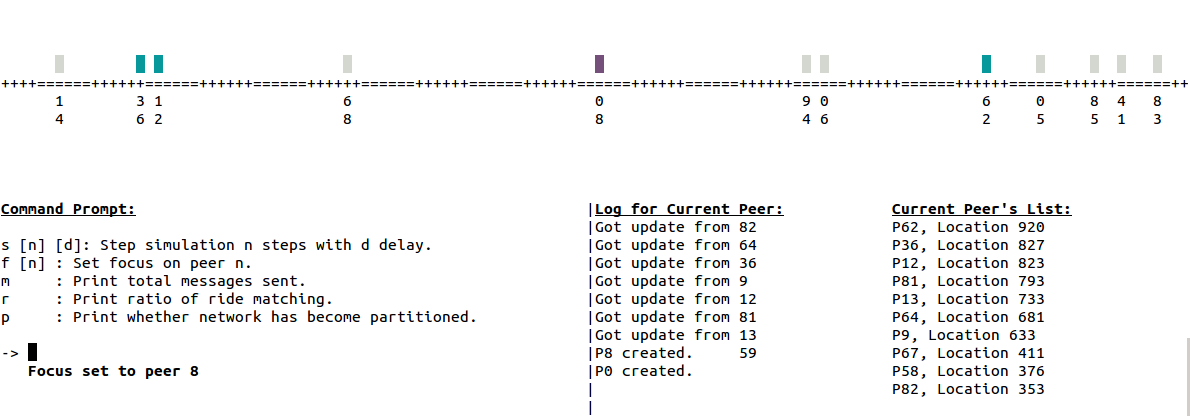
\includegraphics[width=0.9\textwidth]{images/ui.png}     
  \caption{The user interface of our simulator
           \label{ui}}
\end{figure*} 


We wanted to provide a way to visually see how peers were moving around and interacting in the world, so one of the major components of the simulator is a terminal based command prompt and visualizer. See Figure \ref{ui} for a screenshot of the User Interface. The command prompt allows the user to step the simulation forward, set their focus on a different peer, view information about the currently focused peer, and gather various performance metrics. We implemented this fairly complex UI in the terminal using ANSI escape codes which allows you to move the cursor and delete/overwrite text. Thus, every time we step the simulation, we overwrite the updated areas to show the new state. Implementing the UI in the terminal was fairly simple and meant we didn’t need to deal with a GUI library. However, if we were to expand the project and add complexity we would likely want to move out of the terminal to a more full fledged application.

\subsection{Ride-Sharing Protocol}

\begin{figure*}[ht]
  \centering
   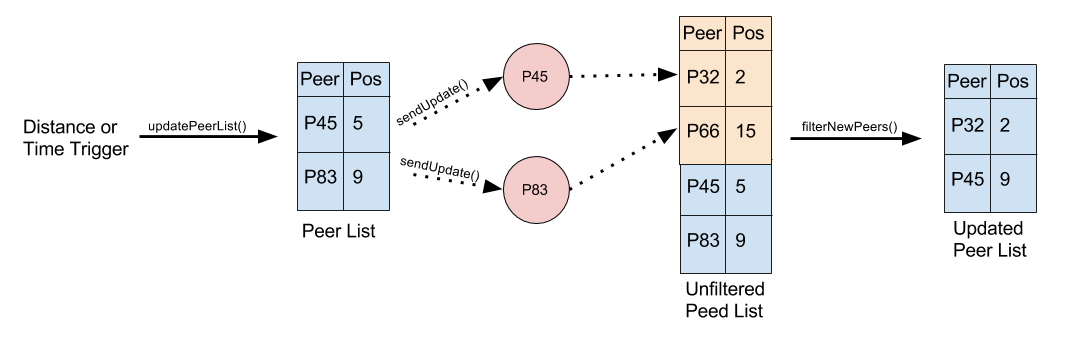
\includegraphics[width=0.9\textwidth]{images/protocol_diagram.png}     
  \caption{Flow of the protocol
           \label{design-diagram}}
\end{figure*} 

Since this is a peer-to-peer system, the core of the service will be the protocol that describes how the peers interact with each other. The protocol we designed leverages the fact that proximity is an important factor in a ride sharing service. 

Figure \ref{design-diagram} demonstrates how the protocol works. To start, when a peer has moved a certain distance or a certain time has elapsed since it sent an update, it will try to contact the peers in its known peer list. The purpose of this contact is to send its updated location to other peers and receive data from the other peers. So the peer it is connecting with will return its list of known peers to the initiating node.


When the initiating peer gets the data from the peers it connected with it now has a longer list of known nodes. We could continue to maintain this longer list, but the tradeoff is that now we will have more peers to communicate with which will result in more message calls over the network, which is undesirable. Thus, we sort all the peers we know about based on proximity and only store a certain number of the one’s closest to us. This is a reasonable tradeoff because it is the peers closest to us that will be most likely to give us a ride, so when it comes time to request a ride we want to know about peers close to us which is what this protocol is designed to capture.

One detail that is not captured in the diagram is that we need to have a way to know what data is fresher when two peers have conflicting information. In other words, if peer A gets information from peer B that peer C is at location x but peer A has information that peer C is at location y, which location should we store and how can we know? To solve this, each peer stores a timestamp along with the location of each peer in its known peer list. Therefore, in the case of a conflict, we simply take the location with the more recent timestamp. Typically, this type of time synchronization can be difficult in a distributed system, but since we are working with mobile devices which should have fairly accurate times from their network providers, and since we need accuracy at the scale of minutes not milliseconds, it seems fair to assume that this method would be effective. 

\begin{figure*}[ht]
  \centering
   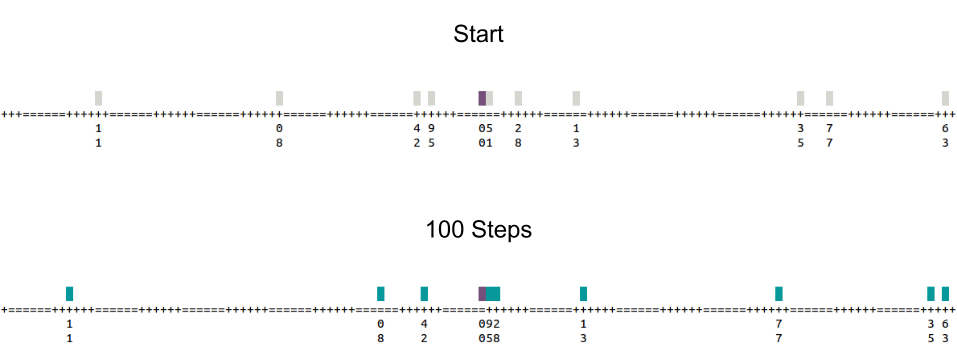
\includegraphics[width=0.9\textwidth]{images/protocol_impact.png}     
  \caption{Suggests the protocol is working as intended as the peers around the focused peer (purple) go from unknown (gray) to known (blue)
           \label{protocol-impact}}
\end{figure*} 


Figure \ref{protocol-impact} indicates that our protocol is working as expected. Our visualization shows that nodes are learning about the peers in close proximity to them which is the aim of the protocol. In the next section we will more closely examine the performance of our protocol. Lastly, to see the code behind our implementation, look at the \texttt{updatePeerList()} method in Peer.scala and to see sample usage of the simulator, see the appendix. 


\section{Evaluation}

\subsection{Baseline vs. Protocol}

Here we evaluate our protocol using our simulator. To start, we ran a series of trials to see how the system performs without a protocol helping to share peer information between the nodes. In other words, these tests help establish baseline metrics that we can compare our protocol against. 

\begin{table}[h]
  \centering
  \begin{tabular}{l || r | r}

  Peer List & Messages & Ratio \\ \hline \hline
  10 Random & 4424216 & 7.42\%  \\ \hline
  Full List & 35556831 & 66.63\% \\ \hline
  Protocol & 5174239 & 65.34\%
  \end{tabular}
  \caption{Baseline results vs. Protocol
    \label{baseline-results}}
\end{table}

The first test we ran has each peer hold a static list of 10\% of the peers in the network. So of the 100 simulated peers, each node holds an unchanging set of 10 random peers. Half of the peers in the network are passengers requesting rides, and passengers request rides with a probability of 10\%. To accept a ride the ride requester and ride offerer have to be within 10 distance units of each other. We ran three trials and each trial ran the simulation for 10,000 steps. Table 1 shows the results. The percentage of fulfilled ride requests was 7.42\% and it took an average of 4,424,216 network messages across all the peers to establish those rides. Clearly, 7.42\% is far too low for a ridesharing service to be usable, no one would use a service that helped them get a ride only 7 out of every 100 rides they request.

The next test tried to simulate the other extreme. Each node holds a complete list of all the peers in the system. This will allow the system to maximize the number of matches, however, maintaining a complete picture of the peer network at each node is certainly not scalable. With these trials, we kept all the conditions the same except for the peer lists. Table 1 shows the results. The percentage of fulfilled ride requests jumped to 66\% which is a much better percentage. However, the number of messages sent jumped by almost 10x to 35,556,831.

These baseline tests help establish concrete goals for our protocol. Namely, we aim to get as close as possible to the 66\% value for ride fulfillment while keeping the number of messages sent and amount of state about the peer network held at each peer down.

As Table 1 shows, when we ran the trials with our protocol implemented, we saw a significant improvement in performance. First, we were able to keep the number of messages sent over the network down very close to the 10 Random Peers condition. Furthermore, despite keeping the messages sent down, we were able to reach a ride servicing ratio that is alomst the same as having the full list of peers known at each peer. Thus, in relation to our baseline numbers, our protocol was extremely effective in this case.

\subsection{Number of Peers and Known Peer List Size}

\begin{figure*}[ht]
  \centering
   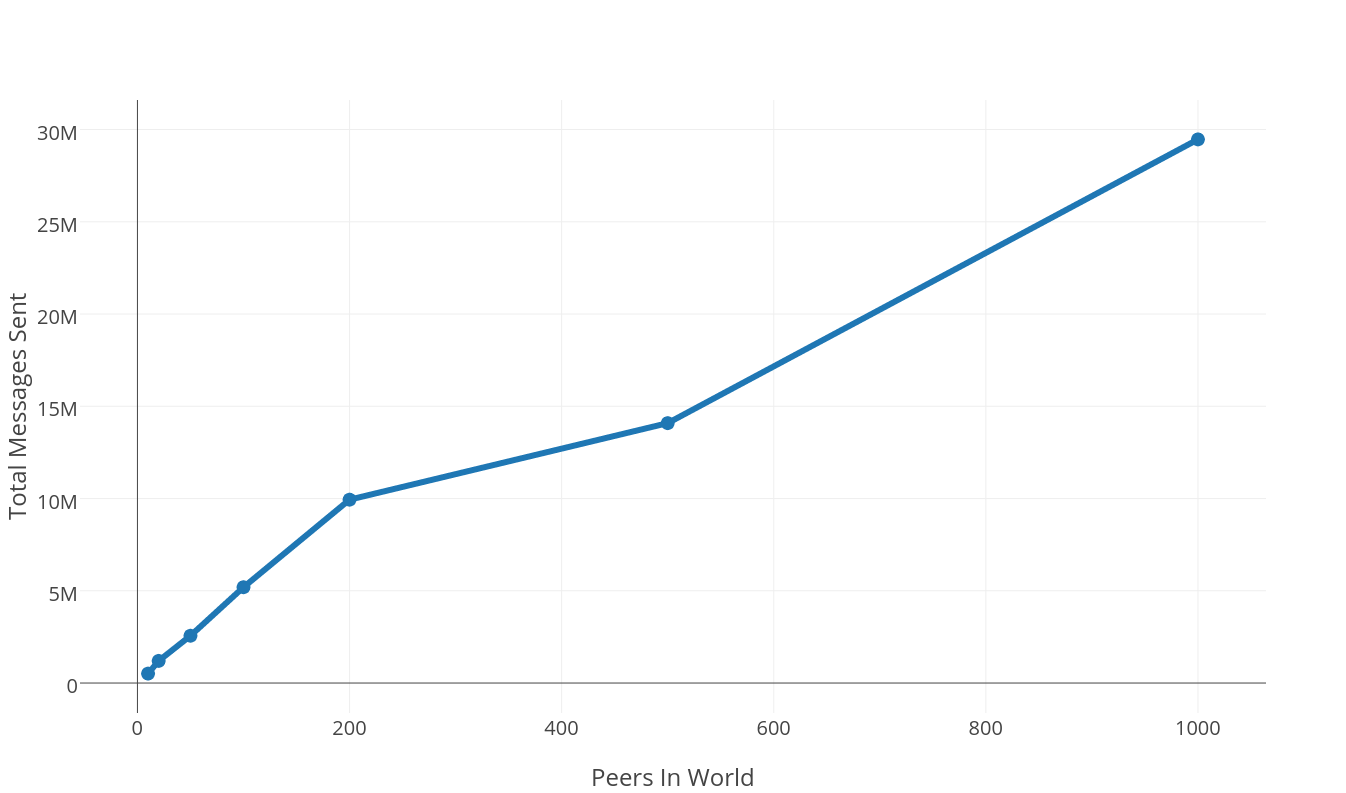
\includegraphics[width=0.9\textwidth]{images/messages_sent_v_peers.png}     
   \caption{Total number of network messages sent after 10,000 steps of the simulator for different number of peers in the world
           \label{messages-v-peers}}
\end{figure*} 

Next we wanted to test how the system scaled as the number of peers in the network increased, so we ran an experiment where we simulated 10,000 steps with 10, 20, 50, 100, 200, 500, and 1000 peers in the network. First, looking at the total number of messages sent shown in Figure \ref{messages-v-peers}, there is a linear increase. This shows that the system is scaling well because it means that, per node, the number of messages getting sent is remaining about the same.

\begin{figure*}[ht]
  \centering
   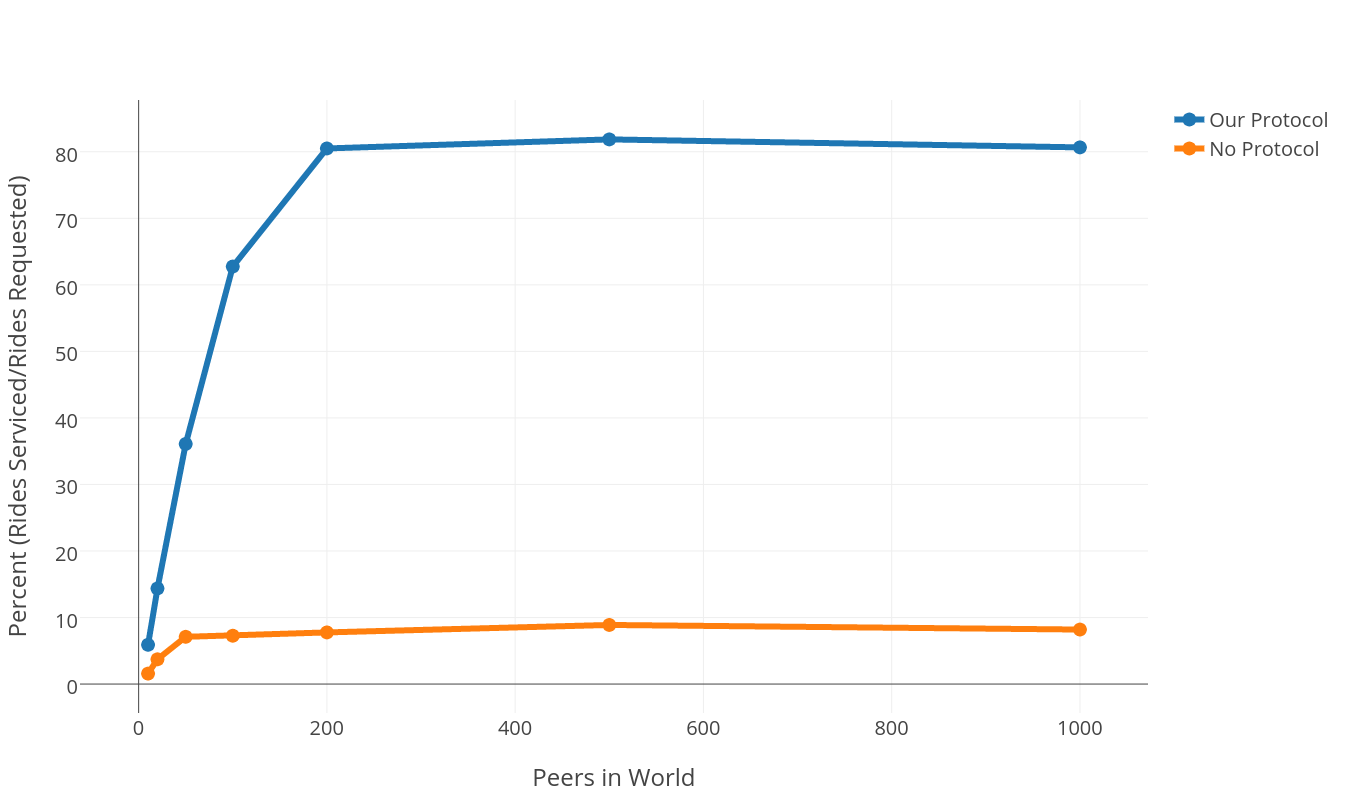
\includegraphics[width=0.9\textwidth]{images/world_density.png}     
   \caption{Percentage of requested rides that were serviced for different number of peers in the world after 10,000 steps of the simulator
           \label{world-density}}
\end{figure*} 

The experiment also shows how the performance of the protocol in terms of matching rides scales. As Figure \ref{world-density} shows, as the number of peers in the world increases, the percent of rides serviced jumps. This is what we want and should expect. As the number of people using the system increases, there are more opportunities to share rides. We included the results of running the experiment without our protocol to show that it is in fact our protocol that is allowing this jump in matches to occur. Without the protocol, the additional opportunities for matches generated by the increased number of peers are not used. \\

\begin{figure*}[ht]
  \centering
   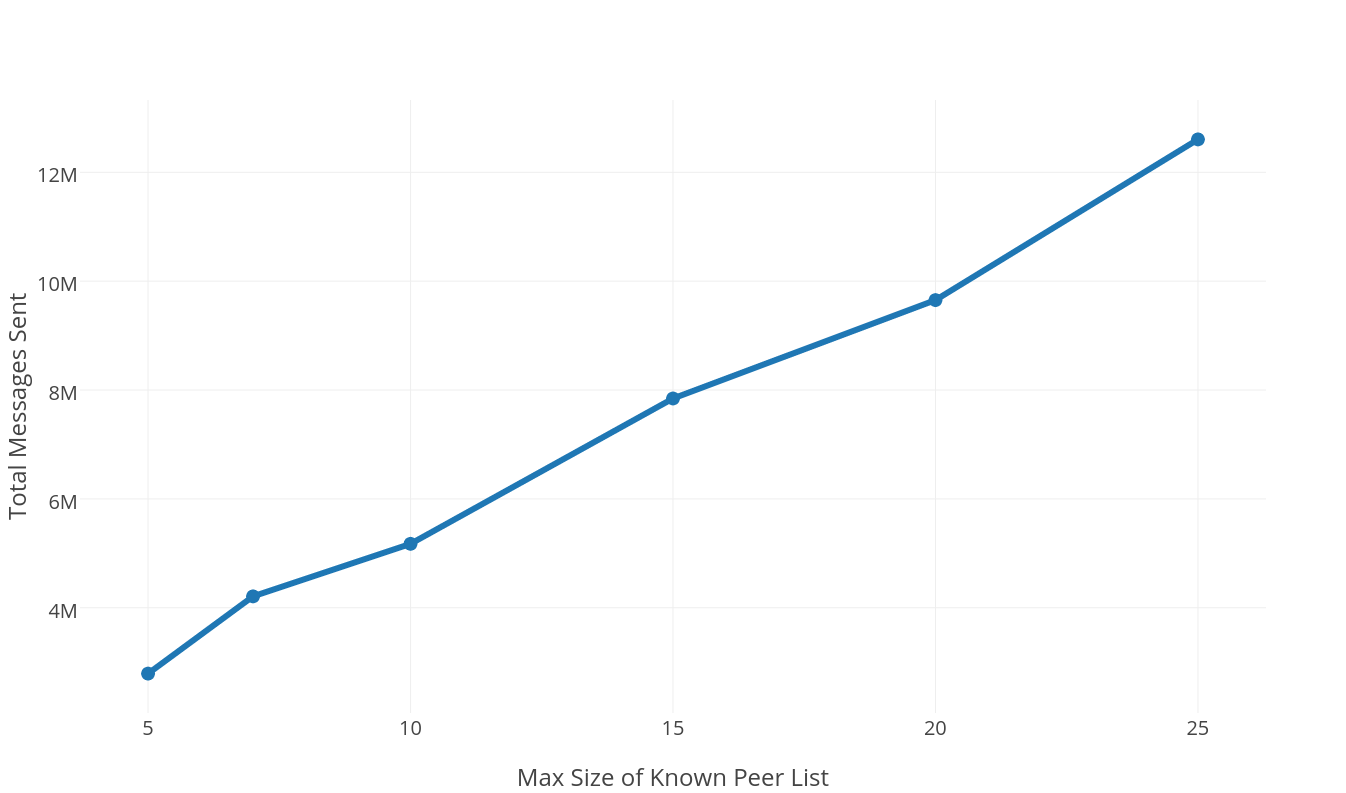
\includegraphics[width=0.9\textwidth]{images/messages_v_pl_size.png}     
   \caption{Total number of network messages sent after 10,000 steps for different Known Peer List sizes
           \label{messages-v-pls}}
\end{figure*} 

\begin{figure*}[ht]
  \centering
   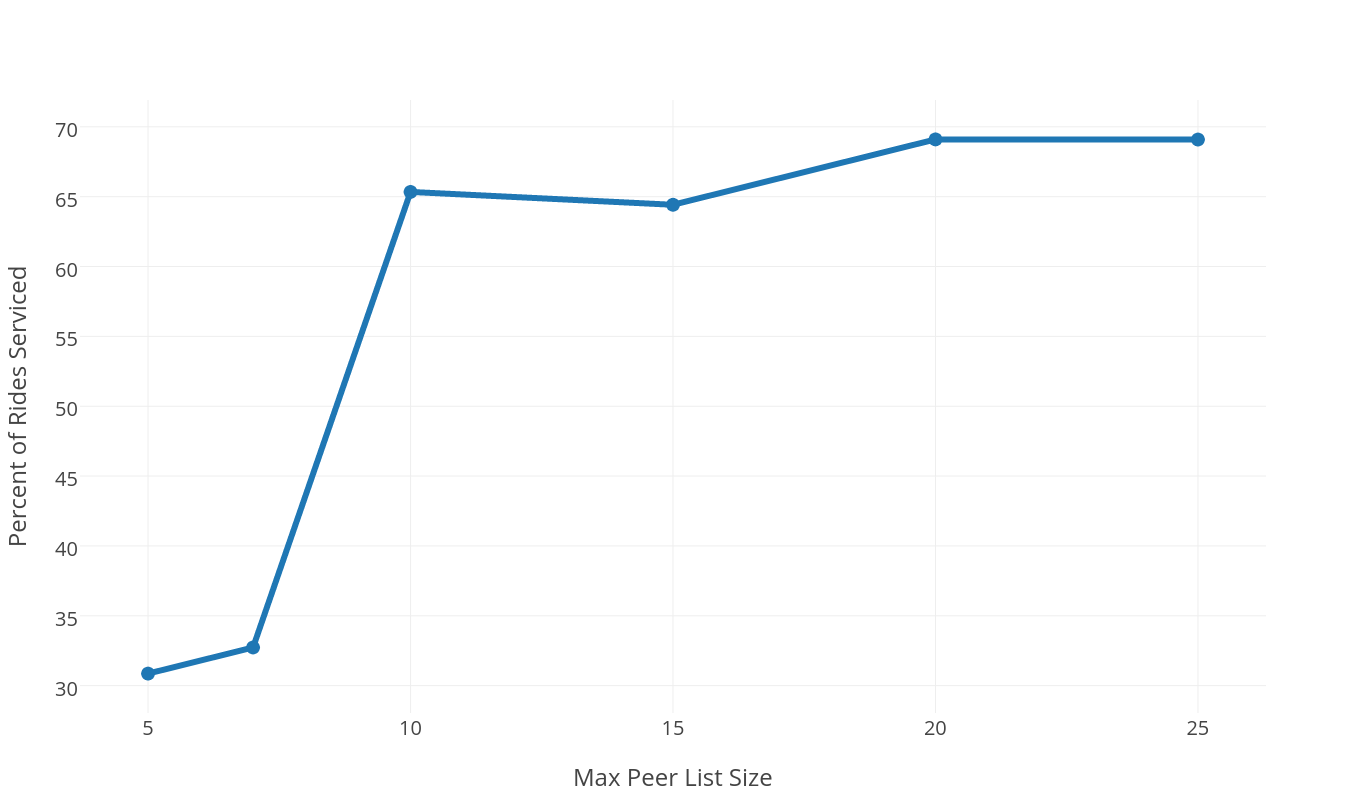
\includegraphics[width=0.9\textwidth]{images/ratio_v_pls.png}     
   \caption{Percentage of requested rides that were serviced after 10,000 steps for different Known Peer List sizes
           \label{ratio-v-pls}}
\end{figure*} 

One of the reasons for developing a simulator was to allow us to quickly see the impact of tweaking certain things in our protocol, so we ran an experiment to demonstrate why that ability to quickly iterate and test things would be useful. The experiment we ran tested the impact of changing the size of the Known Peer List stored at each node. As we discussed, there is a tradeoff involved in keeping a bigger list because a bigger list should allow for more matches but it also means more message sends. We tested Known Peer Lists of size 5, 7, 10, 15, 20, and 25. Figures \ref{messages-v-pls} and \ref{ratio-v-pls} show the results of this experiment. As predicted, the number of messages increases linearly with the size of the list. Thus, it is best to try to keep that list as small as possible. For the percentage of rides serviced, we see that it jumps significantly around 10 and then levels off. This shows that having a Known Peer List of size around 10 is best for this scenario as it maintains matches while keeping messages down.

\subsection{Other Considerations}
Using a partition checking command we implemented in the simulator, we found that after a while, the world would become partitioned into disjoint sub-networks. Our original protocol implementation involved each peer storing locations for only those known nodes that are the smallest distance away. However, because of this, two far away nodes are only prevented from being partitioned by a chaining effect of nodes knowing close by nodes, which know about their close by nodes, and so on. We modified our protocol so that each peer maintains, in addition to its same list of nearby peers, another fixed-size list that contains peers that have become far enough away to fall off the first list. These additional peers provide links between nodes that span different areas of the chain mentioned above. We also tried simply increasing the size of our original peer list. We hypothesized that these changes would help reduce or eliminate partitioning in the system because it adds tighter global connectedness in addition to the tight local connectedness. While we don’t have exact data on the rate of partitioning, we did generally observe that partitioning decreased or at least took many more steps to appear when we included these improvements. We also were able to achieve this reduction in partitioning without increasing the load on the network by very much.

\section{Related Work}
A team in Israel has been working on developing a similarly decentralized real-time ridesharing application called La'Zooz. It appears that La'Zooz is also fully peer-to-peer and additionally incorporates digital cryptocurrency to deal with the issue of free-riding. In a ridesharing system based on payment-free, reciprocal offering and receiving of rides, it is crucial that people do not take without also giving. Without some mechanism for ensuring contribution, this problem would surely manifest because there is no economic incentive to offer a ride for free. La'Zooz clients build up tokens that can later be spent on receiving rides while the user drives around above a certain speed. Because these tokens are a blockchain-based cryptocurrency, they too are inherently peer-to-peer and not able to be faked by a malicious client. Incorporating a payment scheme like this one would be an important consideration going forward with our project.

\section{Future Work}
A critical metric of any distributed system that we did not end up testing much in our system was reliability, and specifically node failure. The one way in which we tested the reliability of the system was in terms of getting it off the ground initially as nodes slowly join. We did this via our more realistic simulation initialization that incrementally adds nodes over time and confirmed that our protocol did allow the network to expand as nodes joined without forming partitions early on in the process. However, node failure is obviously something that every distributed system has to deal with if it is to be successful. It would be important going forward to test our protocol in the presence of failing nodes, especially as nodes are concurrently joining the system as well. Node failures could lead to partitions in the network of peers, so testing if this does occur with our protocol and making improvements to cut down on the chance of this occurring would be key.
                    
Given that we opted to simulate our system for the purposes of this project, there are some important details that have been left out regarding how this system would be actually built for widespread use. Since ridesharing is a primarily mobile application, a full implementation of this service would require thinking much more about what technologies would be best suited for deploying to all types of smartphones, regardless of their platform. Geolocation could be handled nicely using built-in smartphone GPS. Additionally, power consumption is a concern since mobile devices have limited batteries, so going forward we would want to keep this in mind. 

A potential optimization to our location sharing protocol that we did not implement but could prove beneficial in future work is differential sharing based on proximity. This would entail establishing distance thresholds that would determine how frequently updates are communicated between peers and what information is sent back and forth. Peers that are close together would update each other at an increased frequency and with just their location, rather than also sending the peer lists over the network. As peers get farther away from each other, they would send updates less frequently and start to include the peer list on updates beyond a certain distance. This optimization should help to reduce the average message size, thereby reducing bandwidth usage even as total messages sent stays constant.

In this project we decided not to fully implement realistic user behavior upon matching (i.e. the driver moving to the same location as a passenger to pick them up and then the two moving together to a new location). Instead, both driver and passenger simply continue with their own movements but are considered matched and do not match with other peers. While this simplification does not impact any of our measures of interest, it could be worth implementing these behaviors in the future if it became necessary to look more deeply into how user patterns of movement occur or how they impact network characteristics such as partitioning. If these things did become more important, it would be interesting to also incorporate real world data on commuter behavior to improve the movement patterns of our peer groups. We could also look for information regarding differences in real world movement behavior between people in more and less densely crowded regions and apply that to our simulation.

Aside from all of the technical hurdles and design tradeoff decisions presented by the challenge of building a peer-to-peer ridesharing application, there are also a number of security issues that would need to be overcome before such an application could be viable. All of these security problems that we did not explore revolve around the fact that the peer-to-peer nature of the system makes individual users anonymous. Sharing location data with anonymous users could enable stalking or other malicious behavior. Additionally, in an ideal setting the drivers and passengers utilizing a ridesharing service are verified with a background check, for example, and are able to build up a measure of trustworthiness as they use the service without problem. When these users are anonymous, this type of verification would be difficult. Going back to our intended audience of college campuses, however, it may be more feasible to perform a simple verification step. Since college students, faculty, and staff typically have a school-associated email address, the service could be built in instances, one for each campus, and require an email verification step before use can occur on a device.

\section{Conclusions}
This project demonstrated the challenges, complexities, and obstacles involved in building a peer-to-peer network. For one, testing a peer-to-peer system is difficult because the peers make up the entirety of system, so you need many peers for the system to even exist for testing and evaluation. We overcame this problem using a simulator which allowed us to rapidly and easily test our ride-sharing protocol. In writing our simulator and peers, it was important to always be aware of whether we were working on something that was part of the simulator where we could cheat and access global information about our peers, or whether we were essentially pretending to be a peer which has no information aside from what it has learned in the past. We also found that reasoning about a peer-to-peer system is difficult. Since the data is spread over all the peers which are constantly changing state, it is difficult to reason about what state the system is in and what things we can assume. This is unlike a client-server model where it is easier to control and know the state the server. Overall, the project provided a challenging, yet worthwhile experience in working with and reasoning about peer-to-peer systems and protocols.

\appendix
\section{Sample Usage:}

\begin{verbatim}
-> scala -cp bin Simulator -r
...
-> s
\end{verbatim}

After performing one step in the simulation, the central purple peer whose perspective we are taking should be surrounded mainly by gray peers, which are those unknown to the purple peer.

\begin{verbatim}
-> s 100 50
\end{verbatim}

After performing another 100 steps, the majority of visible peers should now be blue, meaning that the purple node is now aware of them. \\

Run without the \texttt{-r} flag to get the incremental initialization that models a more realistic system start-up with new peers joining over time. You will see that after a number of steps, the focused node's peer list becomes populated with known peers.

%\bibliographystyle{plain}
%\bibliography{bibfile}

\end{document}
